% Options for packages loaded elsewhere
\PassOptionsToPackage{unicode}{hyperref}
\PassOptionsToPackage{hyphens}{url}
\documentclass[
]{article}
\usepackage{xcolor}
\usepackage[margin=1in]{geometry}
\usepackage{amsmath,amssymb}
\setcounter{secnumdepth}{5}
\usepackage{iftex}
\ifPDFTeX
  \usepackage[T1]{fontenc}
  \usepackage[utf8]{inputenc}
  \usepackage{textcomp} % provide euro and other symbols
\else % if luatex or xetex
  \usepackage{unicode-math} % this also loads fontspec
  \defaultfontfeatures{Scale=MatchLowercase}
  \defaultfontfeatures[\rmfamily]{Ligatures=TeX,Scale=1}
\fi
\usepackage{lmodern}
\ifPDFTeX\else
  % xetex/luatex font selection
\fi
% Use upquote if available, for straight quotes in verbatim environments
\IfFileExists{upquote.sty}{\usepackage{upquote}}{}
\IfFileExists{microtype.sty}{% use microtype if available
  \usepackage[]{microtype}
  \UseMicrotypeSet[protrusion]{basicmath} % disable protrusion for tt fonts
}{}
\makeatletter
\@ifundefined{KOMAClassName}{% if non-KOMA class
  \IfFileExists{parskip.sty}{%
    \usepackage{parskip}
  }{% else
    \setlength{\parindent}{0pt}
    \setlength{\parskip}{6pt plus 2pt minus 1pt}}
}{% if KOMA class
  \KOMAoptions{parskip=half}}
\makeatother
\usepackage{color}
\usepackage{fancyvrb}
\newcommand{\VerbBar}{|}
\newcommand{\VERB}{\Verb[commandchars=\\\{\}]}
\DefineVerbatimEnvironment{Highlighting}{Verbatim}{commandchars=\\\{\}}
% Add ',fontsize=\small' for more characters per line
\usepackage{framed}
\definecolor{shadecolor}{RGB}{248,248,248}
\newenvironment{Shaded}{\begin{snugshade}}{\end{snugshade}}
\newcommand{\AlertTok}[1]{\textcolor[rgb]{0.94,0.16,0.16}{#1}}
\newcommand{\AnnotationTok}[1]{\textcolor[rgb]{0.56,0.35,0.01}{\textbf{\textit{#1}}}}
\newcommand{\AttributeTok}[1]{\textcolor[rgb]{0.13,0.29,0.53}{#1}}
\newcommand{\BaseNTok}[1]{\textcolor[rgb]{0.00,0.00,0.81}{#1}}
\newcommand{\BuiltInTok}[1]{#1}
\newcommand{\CharTok}[1]{\textcolor[rgb]{0.31,0.60,0.02}{#1}}
\newcommand{\CommentTok}[1]{\textcolor[rgb]{0.56,0.35,0.01}{\textit{#1}}}
\newcommand{\CommentVarTok}[1]{\textcolor[rgb]{0.56,0.35,0.01}{\textbf{\textit{#1}}}}
\newcommand{\ConstantTok}[1]{\textcolor[rgb]{0.56,0.35,0.01}{#1}}
\newcommand{\ControlFlowTok}[1]{\textcolor[rgb]{0.13,0.29,0.53}{\textbf{#1}}}
\newcommand{\DataTypeTok}[1]{\textcolor[rgb]{0.13,0.29,0.53}{#1}}
\newcommand{\DecValTok}[1]{\textcolor[rgb]{0.00,0.00,0.81}{#1}}
\newcommand{\DocumentationTok}[1]{\textcolor[rgb]{0.56,0.35,0.01}{\textbf{\textit{#1}}}}
\newcommand{\ErrorTok}[1]{\textcolor[rgb]{0.64,0.00,0.00}{\textbf{#1}}}
\newcommand{\ExtensionTok}[1]{#1}
\newcommand{\FloatTok}[1]{\textcolor[rgb]{0.00,0.00,0.81}{#1}}
\newcommand{\FunctionTok}[1]{\textcolor[rgb]{0.13,0.29,0.53}{\textbf{#1}}}
\newcommand{\ImportTok}[1]{#1}
\newcommand{\InformationTok}[1]{\textcolor[rgb]{0.56,0.35,0.01}{\textbf{\textit{#1}}}}
\newcommand{\KeywordTok}[1]{\textcolor[rgb]{0.13,0.29,0.53}{\textbf{#1}}}
\newcommand{\NormalTok}[1]{#1}
\newcommand{\OperatorTok}[1]{\textcolor[rgb]{0.81,0.36,0.00}{\textbf{#1}}}
\newcommand{\OtherTok}[1]{\textcolor[rgb]{0.56,0.35,0.01}{#1}}
\newcommand{\PreprocessorTok}[1]{\textcolor[rgb]{0.56,0.35,0.01}{\textit{#1}}}
\newcommand{\RegionMarkerTok}[1]{#1}
\newcommand{\SpecialCharTok}[1]{\textcolor[rgb]{0.81,0.36,0.00}{\textbf{#1}}}
\newcommand{\SpecialStringTok}[1]{\textcolor[rgb]{0.31,0.60,0.02}{#1}}
\newcommand{\StringTok}[1]{\textcolor[rgb]{0.31,0.60,0.02}{#1}}
\newcommand{\VariableTok}[1]{\textcolor[rgb]{0.00,0.00,0.00}{#1}}
\newcommand{\VerbatimStringTok}[1]{\textcolor[rgb]{0.31,0.60,0.02}{#1}}
\newcommand{\WarningTok}[1]{\textcolor[rgb]{0.56,0.35,0.01}{\textbf{\textit{#1}}}}
\usepackage{longtable,booktabs,array}
\usepackage{calc} % for calculating minipage widths
% Correct order of tables after \paragraph or \subparagraph
\usepackage{etoolbox}
\makeatletter
\patchcmd\longtable{\par}{\if@noskipsec\mbox{}\fi\par}{}{}
\makeatother
% Allow footnotes in longtable head/foot
\IfFileExists{footnotehyper.sty}{\usepackage{footnotehyper}}{\usepackage{footnote}}
\makesavenoteenv{longtable}
\usepackage{graphicx}
\makeatletter
\newsavebox\pandoc@box
\newcommand*\pandocbounded[1]{% scales image to fit in text height/width
  \sbox\pandoc@box{#1}%
  \Gscale@div\@tempa{\textheight}{\dimexpr\ht\pandoc@box+\dp\pandoc@box\relax}%
  \Gscale@div\@tempb{\linewidth}{\wd\pandoc@box}%
  \ifdim\@tempb\p@<\@tempa\p@\let\@tempa\@tempb\fi% select the smaller of both
  \ifdim\@tempa\p@<\p@\scalebox{\@tempa}{\usebox\pandoc@box}%
  \else\usebox{\pandoc@box}%
  \fi%
}
% Set default figure placement to htbp
\def\fps@figure{htbp}
\makeatother
\setlength{\emergencystretch}{3em} % prevent overfull lines
\providecommand{\tightlist}{%
  \setlength{\itemsep}{0pt}\setlength{\parskip}{0pt}}
\usepackage{bookmark}
\IfFileExists{xurl.sty}{\usepackage{xurl}}{} % add URL line breaks if available
\urlstyle{same}
\hypersetup{
  pdftitle={Tarea-Examen 4: Simulación Estocástica},
  pdfauthor={José Jorge Martínez de la Cruz},
  hidelinks,
  pdfcreator={LaTeX via pandoc}}

\title{Tarea-Examen 4: Simulación Estocástica}
\author{José Jorge Martínez de la Cruz}
\date{2026-05-18}

\begin{document}
\maketitle

{
\setcounter{tocdepth}{3}
\tableofcontents
}
\begin{Shaded}
\begin{Highlighting}[]
\CommentTok{\# Librerías necesarias}
\FunctionTok{library}\NormalTok{(quantmod)}
\FunctionTok{library}\NormalTok{(xts)}
\FunctionTok{library}\NormalTok{(rugarch)}
\FunctionTok{library}\NormalTok{(copula)}
\FunctionTok{library}\NormalTok{(ggplot2)}
\FunctionTok{library}\NormalTok{(dplyr)}
\FunctionTok{library}\NormalTok{(tidyr)}
\FunctionTok{library}\NormalTok{(knitr)}
\FunctionTok{library}\NormalTok{(gridExtra)}

\FunctionTok{set.seed}\NormalTok{(}\DecValTok{236}\NormalTok{)}
\end{Highlighting}
\end{Shaded}

\subsection{Instrucciones:}\label{instrucciones}

Para cada ejercicio, explique el algoritmo y de el código
correspondiente. Considerando dos series correlacionadas del ejercicio 4
de la Tarea Examen 2

\begin{Shaded}
\begin{Highlighting}[]
\CommentTok{\# vamos a descargar datos de META/Facebook (META) y Apple (AAPL) para el mismo periodo de tiempo (200 días)}
\NormalTok{symbols }\OtherTok{\textless{}{-}} \FunctionTok{c}\NormalTok{(}\StringTok{"META"}\NormalTok{, }\StringTok{"AAPL"}\NormalTok{)}
\FunctionTok{getSymbols}\NormalTok{(symbols, }\AttributeTok{from =} \FunctionTok{Sys.Date}\NormalTok{() }\SpecialCharTok{{-}} \DecValTok{350}\NormalTok{, }\AttributeTok{to =} \FunctionTok{Sys.Date}\NormalTok{(), }\AttributeTok{periodicity =} \StringTok{"daily"}\NormalTok{)}
\end{Highlighting}
\end{Shaded}

\begin{verbatim}
## [1] "META" "AAPL"
\end{verbatim}

\begin{Shaded}
\begin{Highlighting}[]
\CommentTok{\# últimos 200 precios de cierre}
\NormalTok{precios\_meta }\OtherTok{\textless{}{-}} \FunctionTok{as.numeric}\NormalTok{(}\FunctionTok{tail}\NormalTok{(}\FunctionTok{Cl}\NormalTok{(META), }\DecValTok{200}\NormalTok{))}
\NormalTok{precios\_aapl }\OtherTok{\textless{}{-}} \FunctionTok{as.numeric}\NormalTok{(}\FunctionTok{tail}\NormalTok{(}\FunctionTok{Cl}\NormalTok{(AAPL), }\DecValTok{200}\NormalTok{))}
\end{Highlighting}
\end{Shaded}

\subsection{Ejercicio 1}\label{ejercicio-1}

Haga una prueba Ljung Box con lags 5, 10 y 15 individualmente para ver
si los datos pueden considerarse como una muestra, posteriormente
considere los rendimientos logarítmicos y adicionalmente a la prueba
Ljung Box haga una prueba Akaike y grafique las funciones de
autocorrelación para los lags antes mencionados.

\subsubsection{Solución}\label{soluciuxf3n}

Primero aplicamos la prueba de Ljung-Box a las series de precios. La
hipótesis nula de esta prueba es que no hay autocorrelación hasta el
rezago especificado. Si el valor-p es pequeño, rechazamos la hipótesis
de no autocorrelación y concluimos que la serie conserva dependencia
temporal.

Después calculamos rendimientos logarítmicos,

\[
R_t = \log(P_t)-\log(P_{t-1}),
\]

y repetimos el análisis sobre estos rendimientos.

Después de realizar las pruebas de hiótesis en ambos precios de META y
AAPL, los valores-p son menores que 0.05, lo que indica que rechazamos
la hipótesis nula de no autocorrelación. Esto sugiere que las series de
precios tienen dependencia temporal y no pueden considerarse como
muestras independientes. Veamos qué sucede con las series de tiempo de
los rendimientos.

Los resultados se presentan en la siguiente tabla:

\begin{longtable}[]{@{}
  >{\raggedright\arraybackslash}p{(\linewidth - 6\tabcolsep) * \real{0.2222}}
  >{\centering\arraybackslash}p{(\linewidth - 6\tabcolsep) * \real{0.2778}}
  >{\centering\arraybackslash}p{(\linewidth - 6\tabcolsep) * \real{0.2778}}
  >{\raggedright\arraybackslash}p{(\linewidth - 6\tabcolsep) * \real{0.2222}}@{}}
\toprule\noalign{}
\begin{minipage}[b]{\linewidth}\raggedright
Activo
\end{minipage} & \begin{minipage}[b]{\linewidth}\centering
Rezago (Lag)
\end{minipage} & \begin{minipage}[b]{\linewidth}\centering
Valor \emph{p}
\end{minipage} & \begin{minipage}[b]{\linewidth}\raggedright
Resultado Ljung-Box (\(\alpha = 0.05\))
\end{minipage} \\
\midrule\noalign{}
\endhead
\bottomrule\noalign{}
\endlastfoot
\textbf{META} & 5 & 0.0671 & No se rechaza \(H_0\) (Independencia) \\
\textbf{META} & 10 & 0.2680 & No se rechaza \(H_0\) (Independencia) \\
\textbf{META} & 15 & 0.1705 & No se rechaza \(H_0\) (Independencia) \\
\textbf{AAPL} & 5 & 0.4976 & No se rechaza \(H_0\) (Independencia) \\
\textbf{AAPL} & 10 & 0.4645 & No se rechaza \(H_0\) (Independencia) \\
\textbf{AAPL} & 15 & 0.5420 & No se rechaza \(H_0\) (Independencia) \\
\end{longtable}

Y los gráficos de las funciones de autocorrelación (ACF y PACF) para los
precios y rendimientos de META y AAPL se presentan a continuación:

\pandocbounded{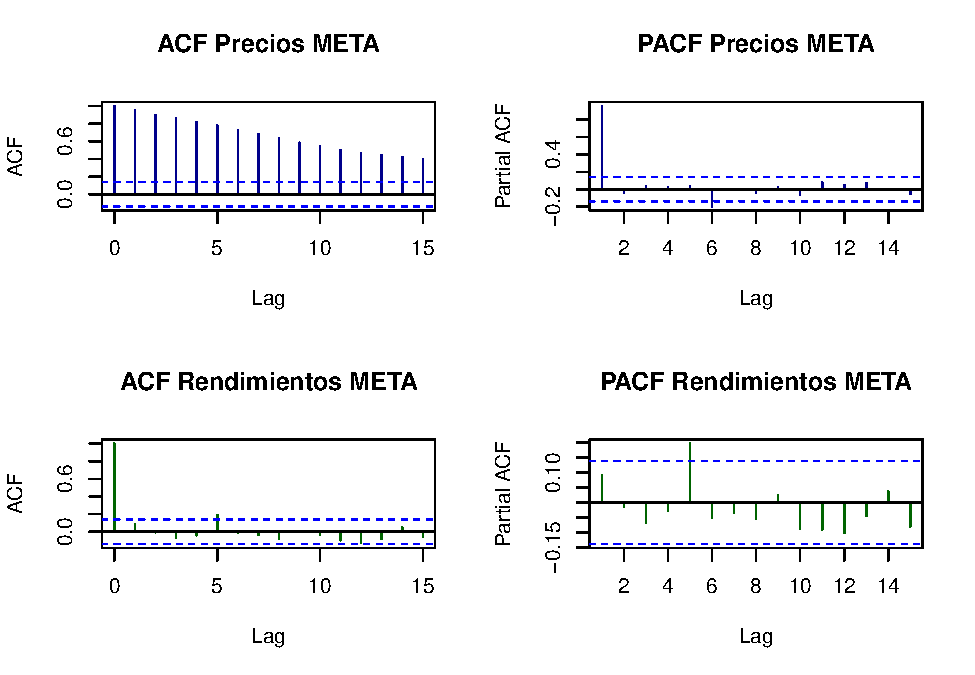
\includegraphics[keepaspectratio]{Tarea_Examen_4_Simulacion_files/figure-latex/unnamed-chunk-7-1.pdf}}
\pandocbounded{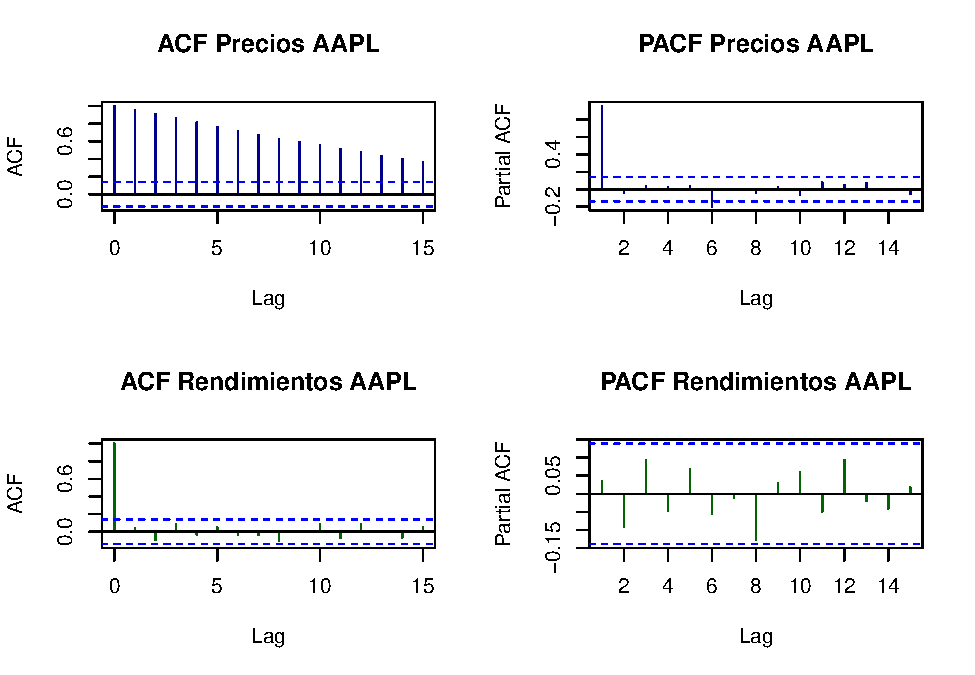
\includegraphics[keepaspectratio]{Tarea_Examen_4_Simulacion_files/figure-latex/unnamed-chunk-7-2.pdf}}

De las gráficas tanto de ACF como de PACF, se observa que existe alta
correlación en los precios originales, hay que notar también que,
aplicar la transformación a los precios para convertirlos a rendimientos
logarítmicos aplica lo siguiente: Una transformación logarítmica para
estabilizar la varianza y una aplicación del operador diferencia para
eliminar la autocorrelación.

\subsection{Ejercicio 2}\label{ejercicio-2}

Genere un ciclo para evaluar distintos parámetros de los modelos
\(ARMA(m,n)- GARCH(p,q)\). Considere \(0 ≤ m, n ≤ 4\) y \(0 ≤ p\),
\(q ≤ 2\) Presente la matriz con los resultados incluyendo las pruebas
estadísticas a los residuales estandarizados de cada modelo así como los
parámetros (ordénela de acuerdo a mayor p-value de la prueba Ljung-Box
promedio). Diga qué modelo escogería para cada una de las dos series y
por qué.

\subsubsection{Solución}\label{soluciuxf3n-1}

Se evaluan modelos ARMA\((m,n)\)-GARCH\((p,q)\) con

\[
  0 \leq m,n \leq 4, \qquad 0 \leq p,q \leq 2.
\]

La parte ARMA modela la media condicional:

\[
  R_t = \mu + \sum_{i=1}^{m}\phi_i R_{t-i} + \sum_{j=1}^{n}\theta_j\varepsilon_{t-j} + \varepsilon_t,
\]

mientras que la parte GARCH modela la varianza condicional:

\[
  \sigma_t^2 = \omega + \sum_{i=1}^{p}\alpha_i\varepsilon_{t-i}^2 + \sum_{j=1}^{q}\beta_j\sigma_{t-j}^2.
\]

Fijaremos como en clase que si uno de los órdenes GARCH es cero y el
otro no, se considera el caso sin GARCH, es decir, GARCH\((0,0)\). Para
cada modelo se guardan:

\begin{itemize}
\tightlist
\item
  los órdenes \(AR, MA, GARCH-p\) y \(GARCH-q\);
\item
  AIC y BIC;
\item
  valor-p de Ljung-Box para residuales estandarizados con rezagos 5, 10
  y 15;
\item
  valor-p promedio de esas tres pruebas;
\item
  valor-p de Ljung-Box para residuales estandarizados al cuadrado.
\end{itemize}

Ordenamos la matriz de resultados de acuerdo con el mayor valor-p
promedio de Ljung-Box sobre residuales estandarizados. La razón es que
valores-p grandes indican menor evidencia de autocorrelación remanente
en los residuales.

Escogemos el modelo de META buscando que los residuales y los residuales
al cuadrado pasen Ljung-Box al nivel 5\%. Si hay varios candidatos, se
escoge el de menor AIC entre ellos. Si ninguno cumple, se toma el
primero de la matriz ordenada.

Y ahora repetimos el mismo proceso para AAPL.

Por construcción, el modelo seleccionado para cada serie es aquel que
deja residuales estandarizados con menor evidencia de autocorrelación.
Además revisamos los residuales al cuadrado, porque éstos ayudan a
detectar si todavía queda dependencia en la volatilidad.En el caso de
los precios de AAPL el modelo usado es \(ARMA(3,4) - GARCH(1,1)\) y en
el caso de META \(ARMA(4,3)-GARCH(2,2)\).

\pandocbounded{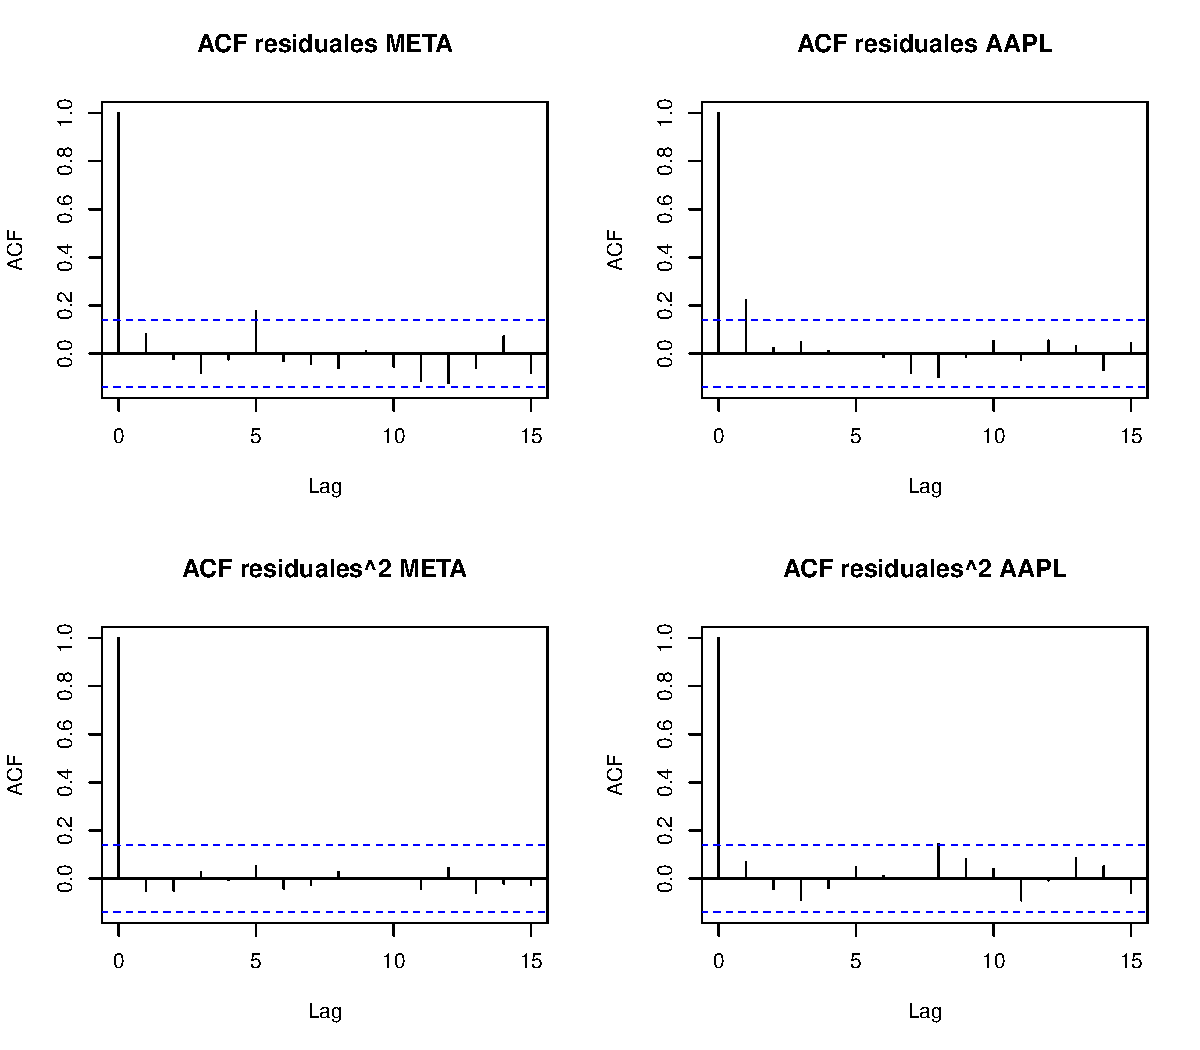
\includegraphics[keepaspectratio]{Tarea_Examen_4_Simulacion_files/figure-latex/ejercicio2-residuales-1.pdf}}

\section{Ejercicio 3}\label{ejercicio-3}

Considerando el modelo óptimo para cada serie, escoja una distribución
para los residuales. Con dicha distribución obtenga la muestra de la
cópula que se utilizará para estimar dicha cópula. Utilizando máxima
verosimilitud estime los parámetros de las cópulas Gaussiana, t de
Student, Gumbel, Clayton y Frank. Utilizando la distancia Cramér-von
Mises con la cópula empírica escoja la mejor.

\subsection{Solución}\label{soluciuxf3n-2}

Usaremos la distribución empírica de los residuales estandarizados. Esto
evita imponer una forma paramétrica adicional a los residuales. Para
construir la muestra de la cópula se transforma cada residual
estandarizado mediante su rango:

\[
U_i = \frac{\operatorname{rango}(z_i)}{N+1}.
\]

Así se obtiene una muestra bivariada en \([0,1]^2\). Y estimamos las
cinco cópulas por máxima verosimilitud.

Para comparar las cópulas se usa la distancia de Cramér-von Mises contra
la cópula empírica. Primero calculamos la cópula empírica en los puntos
observados:

\[
C_N(u_i,v_i)=\frac{1}{N}\sum_{j=1}^{N}\mathbf{1}_{\{U_{j1}\leq u_i,\,U_{j2}\leq v_i\}}.
\]

Luego comparamos esa cantidad con el valor de cada cópula ajustada.Los
resultados se presentan en la siguiente tabla:

\begin{longtable}[]{@{}lc@{}}
\toprule\noalign{}
Cópula & Distancia Cramér-von Mises \\
\midrule\noalign{}
\endhead
\bottomrule\noalign{}
\endlastfoot
\textbf{Gaussiana} & 9.694884e-05 \\
\textbf{t Student} & 9.323047e-05 \\
\textbf{Gumbel} & 1.236233e-04 \\
\textbf{Clayton} & 1.150006e-04 \\
\textbf{Frank} & 1.072208e-04 \\
\end{longtable}

La mejor cópul,a, siguiendo este criterio es la t de Student, aunque la
Gaussiana también se acerca bastante. La diferencia entre ambas es
pequeña, pero la t de Student captura mejor las colas de la distribución
conjunta, lo que puede ser importante para modelar eventos extremos en
los precios de los activos financieros. Por lo tanto, se escogería la
cópula t de Student como la mejor opción para modelar la dependencia
entre los residuales de META y AAPL.

\section{Ejercicio 4}\label{ejercicio-4}

Considerando la cópula Gaussiana, sin importar cuál fue la mejor, y su
parámetro \(\rho\) obtenido vía máxima verosimilitud, junto con la
distribución de los residuales, se construye la distribución conjunta de
los residuales. Obtenga 200 simulaciones normales estándar bivariadas
independientes. Con el método visto en clase genere 200 simulaciones de
la cópula Gaussiana con correlación \(\rho\).

\subsection{Solución}\label{soluciuxf3n-3}

Aunque en el ejercicio anterior se escogió la mejor cópula por distancia
de Cramér-von Mises, aquí usamos obligatoriamente la cópula Gaussiana.
Su parámetro es la correlación \(\rho\) estimada por máxima
verosimilitud.

\begin{verbatim}
##     rho.1 
## 0.3047089
\end{verbatim}

Primero generamos 200 normales estándar bivariadas independientes.
Después inducimos correlación usando la matriz de correlación

\[
\Sigma =
\begin{pmatrix}
1 & \rho \\
\rho & 1
\end{pmatrix}.
\]

Finalmente aplicamos la función de distribución normal estándar
componente a componente para obtener una muestra de la cópula Gaussiana.

\pandocbounded{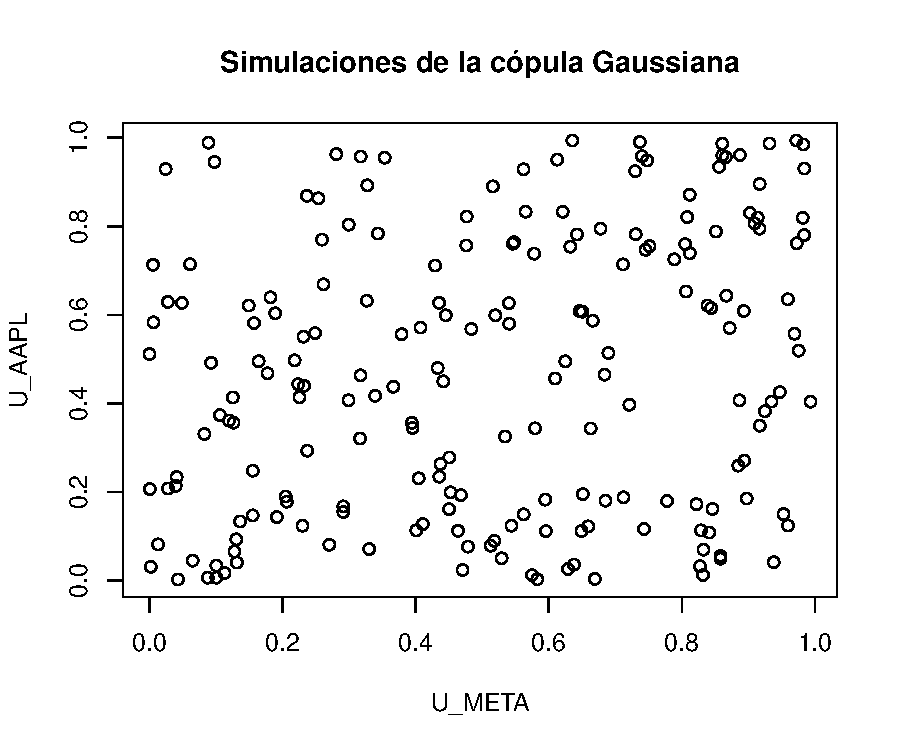
\includegraphics[keepaspectratio]{Tarea_Examen_4_Simulacion_files/figure-latex/unnamed-chunk-16-1.pdf}}

\section{Ejercicio 5}\label{ejercicio-5}

Basado en dicha muestra genere 200 simulaciones de los residuales y 200
simulaciones de los precios originales. Considerando estas últimas
calcule el VaR(95\%) de un portafolio compuesto por 20\% de acciones del
primer activo y 80\% del segundo.

\subsection{Solución}\label{soluciuxf3n-4}

Tomamos las uniformes simuladas de la cópula Gaussiana y las
transformamos a residuales usando los cuantiles empíricos de los
residuales estandarizados de cada activo.

Para pasar de residuales simulados a rendimientos simulados se usa el
pronóstico a un paso de cada modelo ARMA-GARCH:

\[
R_{t+1}^{(sim)} = \widehat{\mu}_{t+1} + \widehat{\sigma}_{t+1} z_{t+1}^{(sim)}.
\]

Después recuperamos precios mediante

\[
P_{t+1}^{(sim)} = P_t \exp(R_{t+1}^{(sim)}).
\]

El portafolio tiene 20\% en META y 80\% en AAPL. Trabajamos con pérdidas
porcentuales simuladas:

\[
L = -\bigl(0.20R_{META}+0.80R_{AAPL}\bigr).
\]

El VaR al 95\% es el percentil 95 de las pérdidas simuladas.

Si se invierte un capital inicial de 1 unidad monetaria, el VaR anterior
se interpreta como pérdida porcentual aproximada. Por ejemplo, para un
capital de 1000 dólares, la estimación es:

\begin{verbatim}
## [1] 29.12653
\end{verbatim}

Finalmente, se grafica el histograma de las pérdidas simuladas del
portafolio, indicando con una línea vertical discontinua el valor del
VaR al 95\%.

\pandocbounded{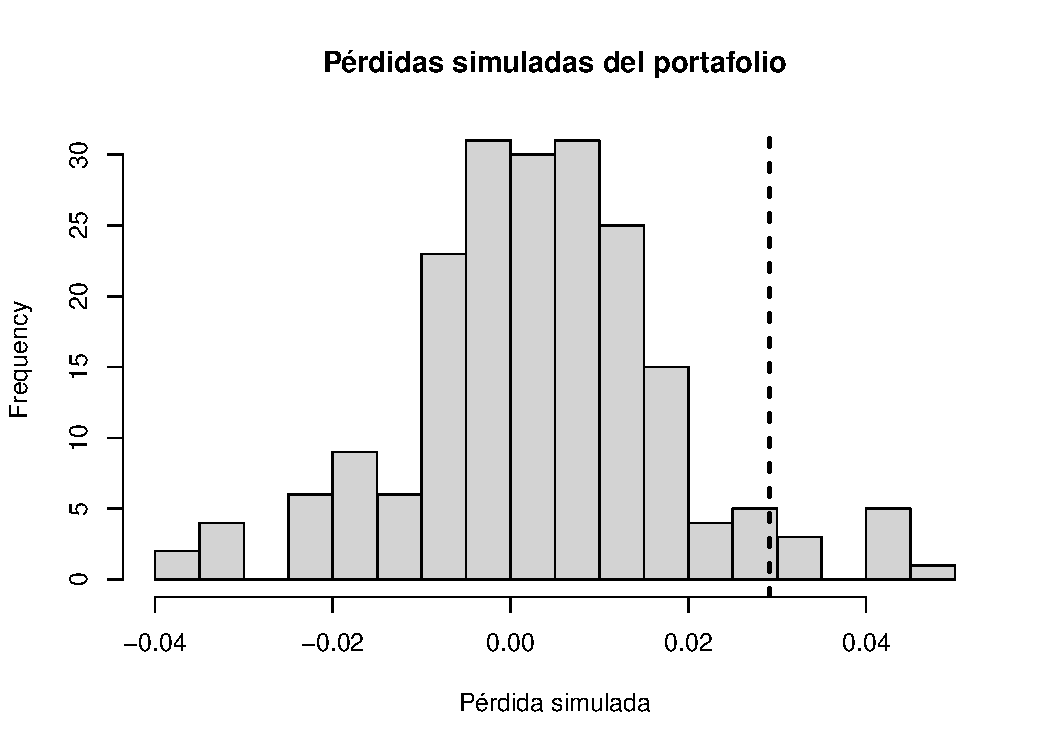
\includegraphics[keepaspectratio]{Tarea_Examen_4_Simulacion_files/figure-latex/unnamed-chunk-20-1.pdf}}

El valor obtenido representa una estimación de la pérdida que no se
excedería con probabilidad aproximada de 95\%, bajo el modelo ARMA-GARCH
marginal y la cópula Gaussiana usada para simular la dependencia entre
los dos activos.

\end{document}
